\documentclass[a4paper]{article}
\usepackage{a4wide}
\usepackage{degeberg}

\title{Principles of Computer System Design \\ Assignment 2}
\author{Daniel Egeberg}

\hypersetup{pdfauthor={Daniel Egeberg},pdftitle={Principles of Computer System Design: Assignment 2}}

\date{December 13, 2012}

\lstset{language=Java}
\setcounter{secnumdepth}{1}
\usetikzlibrary{arrows,shapes}

\newcommand{\mynull}{\textsc{null}}

\begin{document}

\maketitle

\section{Exercises}

\subsection{Question 1: Serializability \& Locking}

\begin{enumerate}[(a)]
    \item The graph for Schedule~1 in \autoref{fig:sched1} has the cycle $T_1
        \to T_2 \to T_3 \to T_1$, so it is not conflict serializable. However,
        Schedule~2 is conflict serializable because the graph in
        \autoref{fig:sched2} is acyclic.

    \item The Strict 2PL protocol only allows conflict serializable schedules,
        so it could not have generated Schedule~1.

        Schedule~2 could not have been generated by Strict 2PL either. Strict
        2PL would grant $T_3$ an exclusive lock on $Z$ and release it when
        $T_3$ commits. However, $T_2$ does a read on $Z$ in between these two
        events. This could not happen as it would require $T_2$ to obtain a
        shared lock while $T_3$ has an exclusive lock on $Z$.

        %Foo\todo{Schedule~2 could probably be made by Strict 2PL. Add the lock operations.}
\end{enumerate}

\begin{figure}[h]
    \centering
    \subfloat[Schedule 1.]{
        \label{fig:sched1}
        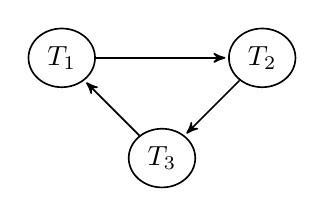
\begin{tikzpicture}
            [->,>=stealth',shorten >=1pt,auto,node distance=1.8cm,semithick]

            \node (t3) [ellipse,draw] {$T_3$};
            \node (t1) [ellipse,draw,above left of=t3] {$T_1$};
            \node (t2) [ellipse,draw,above right of=t3] {$T_2$};

            \path (t1) edge node {} (t2);
            \path (t2) edge node {} (t3);
            \path (t3) edge node {} (t1);
        \end{tikzpicture}
    }\hspace{3em}
    \subfloat[Schedule 2.]{
        \label{fig:sched2}
        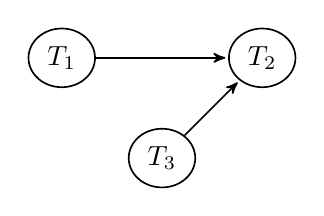
\begin{tikzpicture}
            [->,>=stealth',shorten >=1pt,auto,node distance=1.8cm,semithick]

            \node (t3) [ellipse,draw] {$T_3$};
            \node (t1) [ellipse,draw,above left of=t3] {$T_1$};
            \node (t2) [ellipse,draw,above right of=t3] {$T_2$};

            \path (t3) edge node {} (t2);
            \path (t1) edge node {} (t2);
        \end{tikzpicture}
    }
    \caption{Precedence graphs.}
    \label{fig:precedence_graph}
\end{figure}

%\begin{figure}
%    \centering
%    %\begin{tabular}{lcccccc}
%    %    $T_1$: & S($X$) &               & & & X($Y$) W($Y$) C U($X$) U($Y$) & \\
%    %    $T_2$: &        & & S($Z$) R($Z$) & & & foo \\
%    %    $T_3$: &        & X($Z$) W($Z$) & & C U($Z$) \\
%    %\end{tabular}
%
%    \begin{tabular}{ccc}
%        $T_1$ & $T_2$ & $T_3$ \\
%        S(X) \\
%        R(X) \\
%        && X(Z) \\
%        && W(Z) \\
%        & S(
%    \end{tabular}
%\end{figure}

\subsection{Question 2: Optimistic Concurrency Control}

\begin{description}
    \item[Scenario 1] $T_3$ needs to roll back. Condition~1 fails because $T_2$
        is not done before $T_3$. Conditions~2 and 3 fail because $WS(T_2) \cap
        RS(T_3) = \{4\}$.
    \item[Scenario 2] $T_3$ needs to roll back. Because $WS(T_1) \cap RS(T_3) =
        \{3\}$ thus not satisfying condition~2 or 3 for $T_1$. Condition~1 is
        not satisfied for $T_1$ because $T_3$ begins before it is entirely
        completed.
    \item[Scenario 3] $T_3$ may commit because condition~2 is satisfied for
        both $T_1$ and $T_2$ seeing as $(WS(T_1) \cup WS(T_2)) \cap RS(T_3) =
        \emptyset$.
\end{description}

\subsection{Question 3: Recovery Concepts}

\begin{enumerate}[(a)]
    \item When using force and no-steal, the \textsc{Redo} is not necessary
        because we are guaranteed that the changes are written to disk.
        However, \textsc{Undo} is not necessary either because we are ensured
        that we only writes on commit, and nobody steals the page.
    \item Non-volatile storage retains the stored information when powered
        down, such as a regular HDD\@. This is unlike volatile storage/memory
        like RAM, that requires power at all time to retain the data.

        Stable storage is non-volatile storage that also ensures atomicity of
        write operations. In it should survive any kind of failure, but this
        can obviously not be done perfectly in practice.
    \item In Write-Ahead Loggin (WAL), we need to force a log write when doing
        a commit and doing an update. This is necessary because whenever we
        change things, we want to make sure that we are able to undo it later
        in case the server crashes.
\end{enumerate}

\subsection{Question 4: ARIES}

\begin{itemize}
    \item Winner transactions: $\{T_3\}$
    \item Loser transactions: $\{T_1, T_2\}$
    \item Start of Redo: 3 (the smallest recLSN)
    \item Stop of Undo: 3
    \item Undone LSNs: $\{3, 4, 5, 8, 9\}$
    %\item Rewritten pages: $\{P_1, P_2, P_3, P_5\}$
    \item LSNs that rewrite pages during redo: $\{3,4,5,6,8,9\}$
\end{itemize}

\begin{table}[h]
    \centering
    \subfloat[Dirty page table after analysis.]{
    \begin{tabular}{l|l}
        \toprule
            \textbf{pageID} & \textbf{recLSN} \\
            \midrule
            $P_2$ & 3 \\
            $P_1$ & 4 \\
            $P_5$ & 5 \\
            $P_3$ & 6 \\
            \bottomrule
        \end{tabular}
    }
    \hspace{2mm}
    \subfloat[Transaction table after analysis.]{
        \begin{tabular}{l|l|l}
            \toprule
            \textbf{transID} & \textbf{lastLSN} & \textbf{status} \\
            \midrule
            $T_1$ & 4 & \texttt{U} \\
            $T_2$ & 9 & \texttt{U} \\
            \bottomrule
        \end{tabular}
    } \\
    \subfloat[Final log after \textsc{Undo}.]{
        \begin{tabular}{l|l|l|l|l|l}
            \toprule
            \textbf{LSN} & \textbf{lastLSN} & \textbf{transID} & \textbf{type} & \textbf{pageID} & \textbf{undoNextLSN} \\
            \midrule
            1 & - & - & begin CKPT & - & - \\
            2 & - & - & end CKPT & - & - \\
            3 & \mynull & $T_1$ & update & $P_2$ & - \\
            4 & 3 & $T_1$ & update & $P_1$ & - \\
            5 & \mynull & $T_2$ & update & $P_5$ & - \\
            6 & \mynull & $T_3$ & update & $P_3$ & - \\
            7 & 6 & $T_3$ & commit & - & - \\
            8 & 5 & $T_2$ & update & $P_5$ & - \\
            9 & 8 & $T_2$ & update & $P_3$ & - \\
            10 & 6 & $T_3$ & end & - & - \\
            11 & - & $T_2$ & clr & $P_3$ & 8 \\
            12 & 11 & $T_2$ & clr & $P_5$ & 5 \\
            13 & 12 & $T_2$ & clr & $P_5$ & \mynull \\
            14 & 13 & $T_2$ & end & - & - \\
            15 & - & $T_1$ & clr & $P_1$ & 3 \\
            16 & 15 & $T_1$ & clr & $P_2$ & \mynull \\
            17 & 16 & $T_1$ & end & - & - \\
            \bottomrule
        \end{tabular}
    }
    \caption{Tables resulting from running ARIES.}
\end{table}

\section{Implementation}

\subsection{Question 1}

The logger is implemented in \texttt{MyLogger}.  This takes a log file as a
\texttt{RandomAccessFile} in the constructor. Calling \texttt{logRequest}
creates a \texttt{Future<?>} that writes to the log file. The written contents
are the byte size of the serialized \texttt{LogRequest} followed by the
serialized \texttt{LogRequest} itself. Logging is done in
\texttt{KeyValueBaseImpl} by first performing the write operations where the
data is pinned to memory. Assuming this goes well, we make a log request and
wait until it has been written to disk. It may then later be unpinned and
flushed to the disk by the checkpointer.

The checkpointer in \texttt{MyCheckpointer} takes an instance of
\texttt{KeyValueBaseImpl} and \texttt{IndexImpl}. The checkpointer does the
quiesce-flush-resume loop every every two seconds forever. Quiescing is done by
having a reentrant lock on the entire system. Each operation takes the shared
read lock when running. Quiescing and resuming is then done by taking and
releasing an exclusive write lock. This ensures that no operation will be
admitted while the checkpointer runs.

\subsection{Question 2}

I tested the implementation by first writing some things to the database
ensuring that log records are written. Restarting the server should then replay
the non-empty log file. This can be verified by making a client that reads the
relevant keys.

The system recovers if a log file exists. This means that a database
administrator should remove this file if he wishes to start a fresh server.

\subsection{Question 4}

An obvious way to test the logging overhead would be to measure the performance
with logging disabled and enabled. This is done by having a varying number of
clients (1--500) make simultaneous \texttt{write} requests to the database.

We would definitely like to perform some tests on a computer with much
less/more memory to see the latency de-/increases we expect from the memory
mapped file response times. The number of cores available should also have some
effect.

The Zipf distribution sample keys were generated by the Apache Common Math
library.

The service was tested running on a single Lenovo Thinkpad T420 with the
following specifications:

\begin{itemize}
    \item Intel Core i5-2520M CPU @ 2.50GHz
    \item 8 GB RAM
    \item 256 GB SSD
\end{itemize}

\subsection{Question 5}

The results from the experiment outlined in Question~4 can be seen in
\autoref{fig:latency} and \autoref{fig:throughput}. We observe that the latency
decreases and throughput increases when we disable logging and checkpointing.
This is as expected. With 500 concurrent clients making writes, we observe a
13.5\% overhead in throughput and a 35\% overhead in latency when it is
enabled.

\begin{figure}[h]
    \centering
    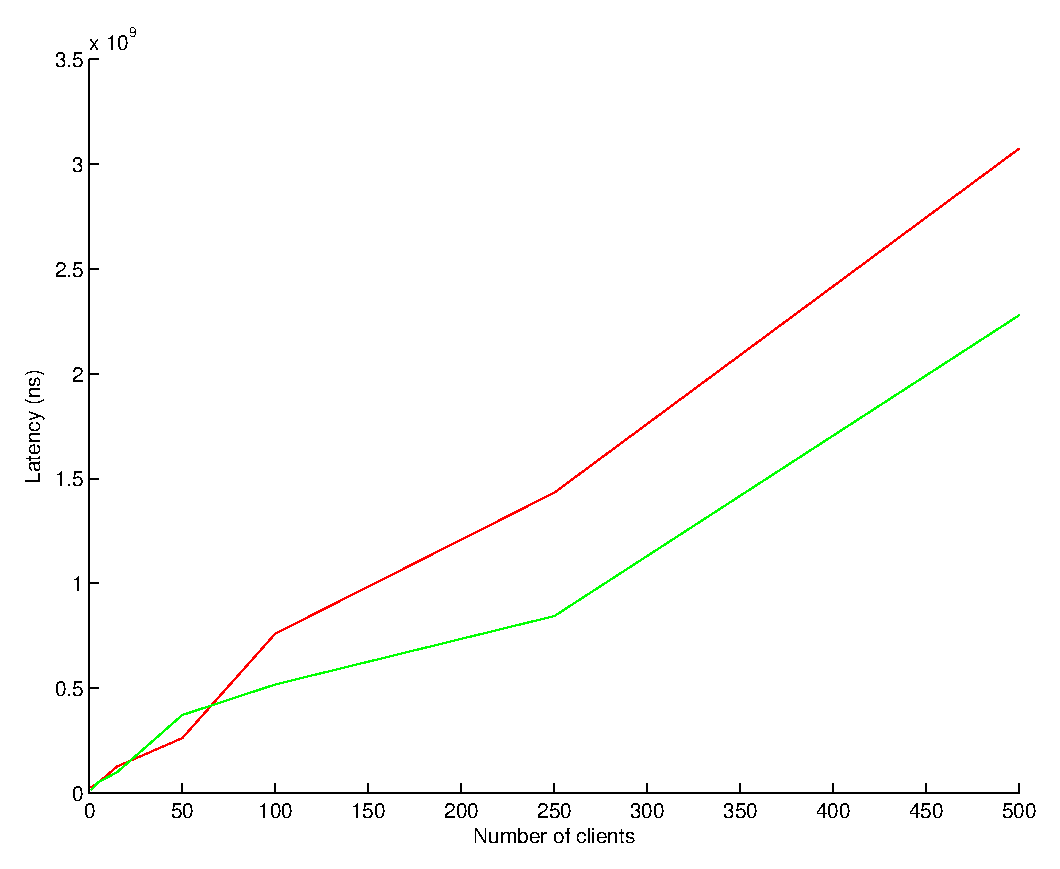
\includegraphics[scale=0.7]{latency}
    \caption{Latency. Red is with logging and checkpointing. Green is without.}
    \label{fig:latency}
\end{figure}

\begin{figure}[h]
    \centering
    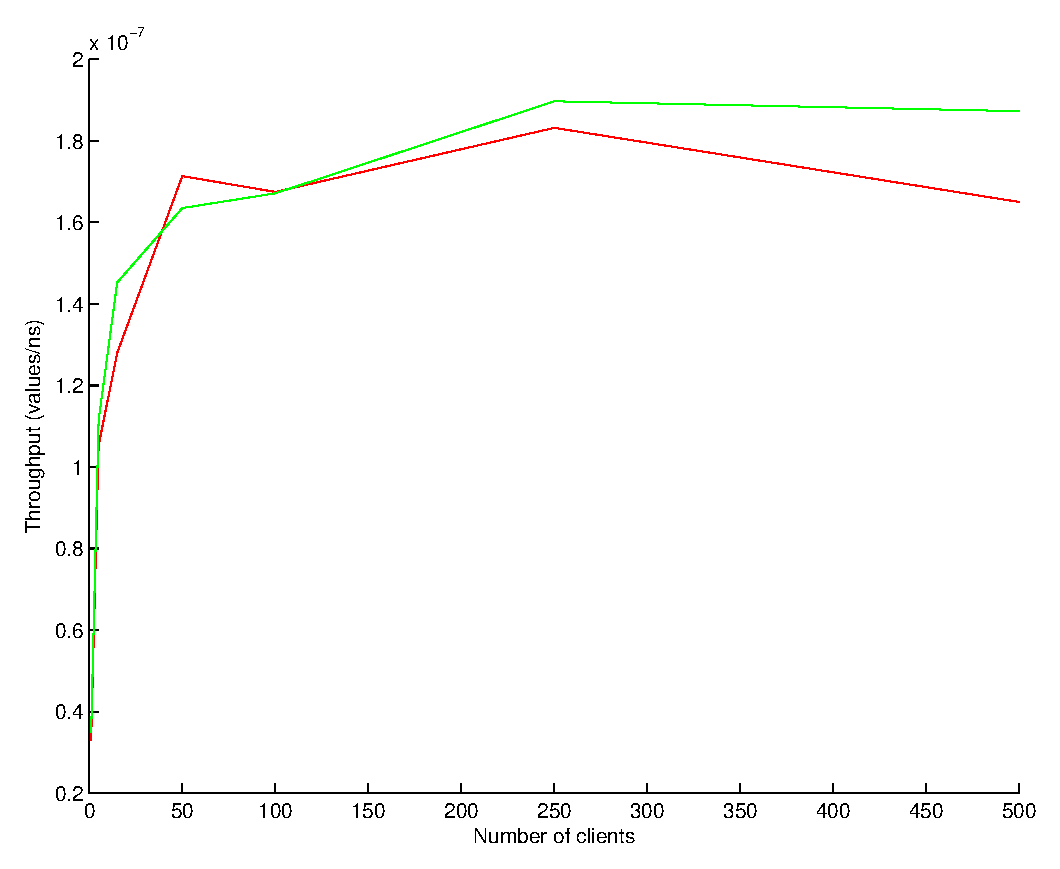
\includegraphics[scale=0.7]{throughput}
    \caption{Throughput. Red is with logging and checkpointing. Green is without.}
    \label{fig:throughput}
\end{figure}

\section{Extensions}

\subsection{Question 6}

I use a thread pool of size \texttt{groupSize} (default is 5) and submit log
write tasks to the executor. The submitted tasks always wait immediately. Each
time we increment \texttt{groupWaiting}. When \texttt{groupWaiting} reaches
\texttt{groupSize} we wake up all threads. A default timeout of 150~ms is added
on the waits to improve performance if there is a low number of concurrent
clients. Threads are woken up using \texttt{notifyAll}. This doesn't actually
ensure that the \texttt{logRequest}s are written in order, but this doesn't
matter as two \texttt{logRequest}s with an overlapping key set cannot be
waiting at the same time. The result of later replaying the log will remain
unchanged no matter the order \texttt{notifyAll} wakes threads.

\end{document}
